% Kapitel 2 - Related Work / Literaturanalyse
\section{Related Work}
This section discusses about game development of educational games, gamification and other tools focused on teaching computational skills but with different game elements and didactic approaches.

\subsection{Gamification and Game-Based Learning}
\cite{10.1145/2181037.2181040} defines gamification as "the use of game design elements in non-game contexts", this increases the engagement of the learner   (CITE HERE). Figure 1 classifies gamification and differentiates it to similar areas. There is a large number of game mechanics that can be added in terms of gamification (Brull and Finlayson, 2016; S. Kim et al., 2018):
\begin{itemize}
    \item Points
    \item Badges
    \item levels
    \item Leaderboards
    \item Progression Bars
    \item Certificates
    \item Story
    \item Avatar (selection and customization)
\end{itemize}

Examples of gamification can be seen in apps like Kahoot! and Duolingo. They are platforms in which lessons and quizes are given out, these are traditional questions that are usually given out in a learning or exam setting, but with now extra unlockables and collectibles. 

\begin{figure}[H]
    \centering
    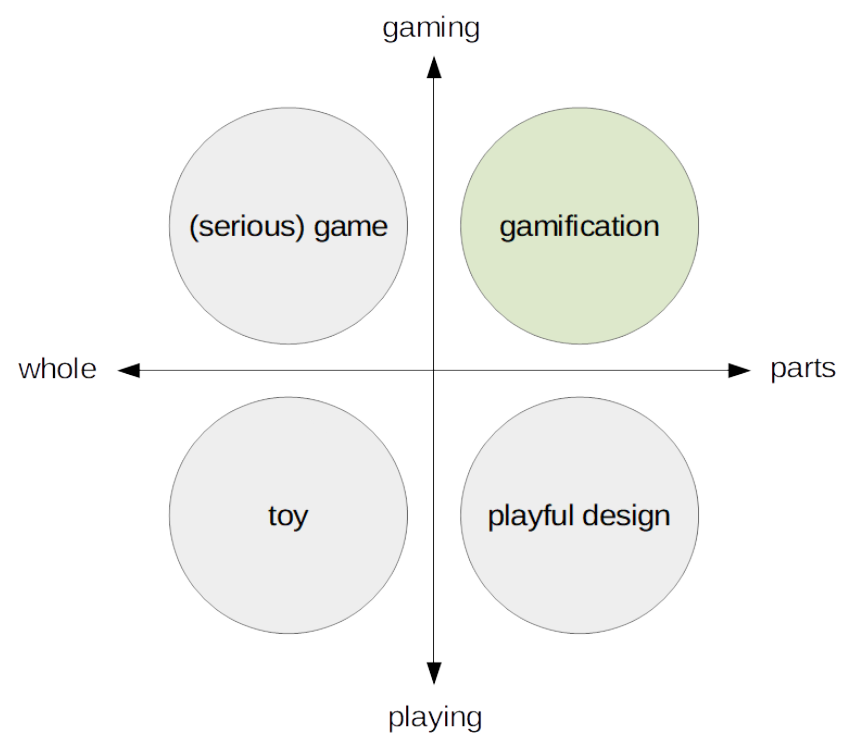
\includegraphics[width=0.5\linewidth]{images/dimensions.png}
    \caption{The dimensions of gaming/playing and whole/parts (After \cite{10.1145/2181037.2181040})}
\end{figure}

In order to distinguish gamification from game-based learning, gamification just introduces gamelike elements (elements or mechanics) into a non-gaming setting. Game-based learning, however, is a type of game play that has defined learning outcomes (Becker, 2021). With a specific learning goal in mind, a learning task is redesigned to make learning more interesting and more effective. This involves the use of serious games and elements of gamification in the learning process, seen as a tool of game-based learning. 

\subsection{Game Frameworks}
To date, educational game development teams have utilized a diverse mix of game design and instructional design methodologies to help realize their designs, but often without a unifying framework to bring these diverse perspectives together. An iterative approach to designing educational games is Winn's (2008) Game Design Play and Experience Framework, which is a modificaiton of the Mechanics, Dynamics, and Aesthetics (MDA) Framework as it does not address aspects outside of Entertainment. According to Figure 1.2, the designer of an educational game would usually have to take into account 4 different layers[17]. Learning, Storytelling, gameplay and user experience. This thesis focuses on the 3rd and 4th layer of the framework, gameplay and user experience.

\begin{figure}[H]
    \centering
    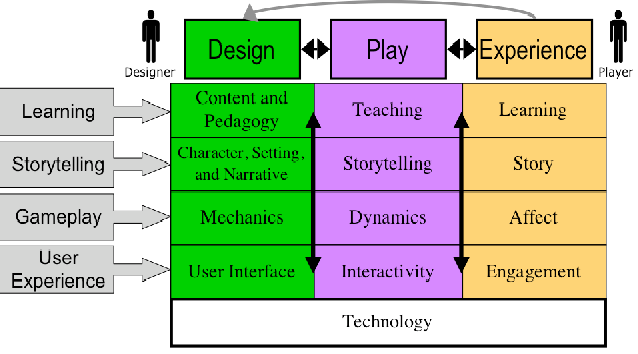
\includegraphics[width=0.5\linewidth]{images/dpe framework.png}
    \caption{Design, play and experience framework}
\end{figure}


The gameplay layer most closely resembles another framework. The gameplay layer defines what the player does in the game and is broken down into mechanics, dynamics and effects. The mechanics are the rules that define the operation of the game world, what the player can do, the challenges the player will face, and the player’s goals. The dynamics are the resulting behavior when the rules are instantiated over time with the influence of the
player’s interactions. The resulting experiences, or emotions derived in the player, are the affects. This is the rules and operations of the game world and the background processes of our game. For the purposes of the project, our focus on executing code is the core mechanic and dynamic of the game.

The user experience layer is designed so that user interfaces are made to access the entertaining gameplay (Saltzman, 2000, p. 256) and to create a vehicle to realize the desired serious outcomes. Good user interfaces are said to be transparent, that is, the player does not have to focus their attention on how to play the game (i.e., what button to press) but rather on the gameplay, storytelling, and learning experience.

The aspects of gameplay and user experience layer of the designer are key areas of game development concern that should also be implemented for educational games. The conceptualisation and implementation of such game elements/mechanics for the project will be explored in depth in later sections.

\subsection{Other educational games in Computer Science}
According to \cite{combefis2016learning}, there are mainly three categories of games in Computer Science:
\begin{itemize}
    \item \textbf{Coding}: The focus is to make users learn and train to code. Coding games require the learner to understand and to be able to write code to solve challenges. A central part is to understand the syntax behind a programming language.
    \item \textbf{Algorithmic thinking}: The focus is not on learning a particular programming language and relating concepts, but on learning concepts like algorithms and data structures. The system provides various problems that have to be solved in a technical way. This does not necessarily use programming languages, but can be done with other concepts.
    \item \textbf{Creating games}:  It is a kind of online programming learning platform that offers the possibility for the users to create their own games. On these platforms, the learner has to program a game, typically with a visual programming language. 
\end{itemize}